\chapter{Geologi}
For at kunne dimensionere et fundament, er det vigtigt at have en grundlæggende viden om det materiale, der arbejdes med, altså hvilken jord, samt dets egenskaber og geologien i området. I det følgende vil der derfor foretages en beskrivelse af Aalborgs geologi, samt en beskrivelse af jorden og dets styrkeparametre.

\section{Jord}
\subsection{Beskrivelse af jord og jordtyper}
Jord er en massebetegnelse, da der findes mange forskellige typer af jordarter. Der findes to hovedgrupper af jord; rene mineraljordarter og organiske jordarter. 
\newline \indent{     }  De rene mineraljordarter kan være sorterede eller usorterede. Mineraljordarterne kan blive sorteret ved vand- og vindaflejring, og kan blive til det, der kendes som grus, sand, silt og ler. De usorterede mineraljordarter aflejres primært ved gletsjeraflejring, og betegnes som morænejordarter kaldet till.\citep{jordarter}
\newline \indent{     }  Organiske jordarter består af organisk materiale i form af plante- eller dyrerester. Disse jordarter kendes som muld, tørv, gytje mm.\citep{miljo}
\newline \indent{     } De forskellige jordtyper kan opdeles i to kategorier; friktionsjord og kohæsionsjord som har forskellige egenskaber. Egenskaberne afhænger af kornstørrelserne, som angives ved kornets diameter, og herved kan de inddeles i kornfraktioner\citep{geoteknik}.De grovkornede jordarter er friktionsjord hvor styrken kommer fra friktion mellem kornene. De finkornede jordarter er kohæsionsjord, hvor styrken skyldes indre sammenhæng mellem kornene.For eksempel ses inddelingen af kornstørrelserne for nogle mineral jordarter på Figur \ref{fig:kornstorrelser} .

\begin{figure}[htbp]	\centering
	\begin{minipage}[b]{0.48\textwidth}
		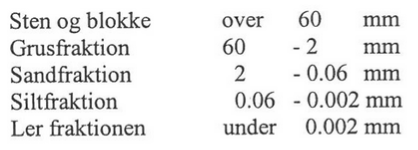
\includegraphics[width=1.0\textwidth]{billeder/kornetsdiameter.png}
		\caption{Inddeling af kornstørrelser for mineraljordarter \citep{jordarter}}
		\label{fig:kornstorrelser}
	\end{minipage}\hfill
\end{figure}

\subsection{Jordtypernes udseende og dannelse}
Grus-  og sandjordarter skabes ved forvitring og erosion af materiale fra faste bjergarter. Materialet bliver herefter transporteret og aflejret via vind eller vand. Dette gør, at deres sammensætning bestemmes af udgangsmaterialet, men i lige så høj grad af transportmåden og transporttiden. Transporttiden kan gøre, at bløde dele af materialet opløses, samt at materialet får en afrundet kornform, og dette giver en mindre friktionsvinkel. Den relative store kornstørrelse ved grus og sandjordarter gør, at de har et groft porenet, hvilket medvirker, at vandet bevæger sig let i materialet,  dvs. at permeabiliteten er stor. Samtidig ved belastning af materialet sker der en vandudpresning, hvilket er en hurtig konsolidering.\citep{jordarter}
\newline \indent{     }  Grus- og sandjordarters styrkeegenskaber afhænger af friktionen mellem kornene, som afhænger af kornenes lejringstæthed, materialets enskornethed og kornenes enkelte form; om de er skarpkantet eller afrundet.\citep{jordarter} 
\newline \indent{     }  Lerjordarter har alle et bestemt indhold af lermineraler. Indholdet af disse har en betydende indflydelse på lerjordartens egenskaber, også selvom de ikke udgør størstedelen af jordarten. Lermineralerne bliver til ved en kemisk forvitring af faste bjergarter. De mest betydende grupper af lermineraler er; kaolinit, smectit, illit og chlorit. Den kemiske sammensætning af lermineralerne kan være meget forskellige og har en stor betydning for de fysiske egenskaber.\citep{jordarter} Alle lermineralerne kan optage vandmolekyler, hvilket gør, at lerjordarter kan indeholde meget vand. Betydningen af vandet kan fysisk ses ved tilsætning af vand til lerjordarterne, som gør at de sveller og ligeledes svinder ved tørring. Hvis lerpartiklerne er placeret med kort afstand til hinanden, vil dette give jordarten en større styrke.\citep{jordarter}  Ved at smadre jordarten formindskes jordartens styrke, men en del af denne styrke kan jordarten genvinde. \citep{jordarter}
\newline \indent{     }  Morænejordarter er typisk usorterede mineraljordarter, og kan derfor bestå af flere forskellige kornstørrelser. Fordelingen af dem kan skifte inden for korte afstande. Morænejordarter har normalt gode styrke- og deformationsegenskaber, da de er forbelastede.\citep{jordarter}
\newline \indent{     }  Organiske jordarters egenskaber er afhængige af de organiske bestanddeles art. De forskellige typer af organiske jordarter bliver dannet forskellige steder. Tørv og gytje bliver for eksempel dannet i moser, søer, bugter, fjorde mm, og dets styrke er ikke høj. Dette skyldes, at disse indeholder store mængder vand, da der ikke er faste partikler og at organiske materialer forsvinder med tiden. \citep{jordarter}

\subsection{Jords styrke og stivhed}
Jord betragtes, ligesom beton og stål osv, som et byggemateriale, da dens fysiske egenskaber er vigtige for konstruktions dimensionering.\citep{DGF} 
\newline \indent{     }  Jordarterne har meget forskellige styrker, og inden for geoteknik kan jordarterne inddeles i to forskellige typer. Den ene type er friktionsjord, for eksempel sand og grus. Den anden er kohæsionsjord med et indhold af mere end 10\% lerfraktion. 
Friktionsjord er under stabil lejring næsten usammentrykkeligt, og hvis deformationer finder sted forskydninger eller gnidninger kornene imellem.\citep{DGF}
\newline \indent{     }  I kohæsionsjord kan kornskelettet være stabilt ved åbne strukturer, men kun ved små deformationer og belastninger, afhængig af forbelastning. Ved store belastninger er disse jordarter sammentrykkelige.
\newline \indent{     }  Med hensyn til jordarters styrke, benyttes begreberne træk- og trykstyrke normalvis ikke. I stedet anvendes forskydningsstyrken. Denne anvendes da der ved brud i jorden, sker en forskydning af jordmasser. Når der sker et sådant brud, virker der normal- og forskydningsspændinger langs brudlinjen.\citep{geoteknik} Forskydningsspændingen $\tau_f$ virker som en reaktion på jordmassens bevægelse nedad, og derfor er denne rettet skråt op ad. Normalspændingen $\sigma_f$, også kaldet brudspændingen, står vinkelret på brudlinjen, og regnes positiv ved tryk \citep{geoteknik}. Dette er illustreret på Figur \ref{fig:poretrykket}. 

\begin{figure}[htbp] \centering
	\begin{minipage}[b]{0.48\textwidth}\centering
		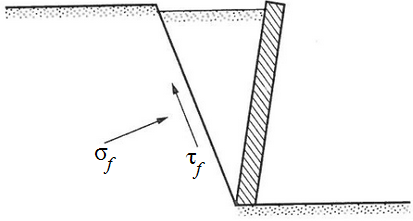
\includegraphics[width=1.0\textwidth]{billeder/poretrykket.png}
		\caption{Brud af jord \citep{Geoteknik}}
		\label{fig:poretrykket}
	\end{minipage}\hfill
\end{figure}

For at finde styrken i jord laves et triakselforsøg, der laves via et triaksialapparat, dette er illustreret på Figur \ref{fig:forskudningsspanding}. Forsøget er det mest anvendte for at finde jords styrke. En cylindrisk jordprøve tilpasses så den har samme diameter som højde. Prøven indsættes lodret i apparatet og indesluttes en tæt gummimembran. Trykhoveder er placeret på prøvens ender, disse er gjort næsten helt glatte vha. siliconesmurte gummihinder, der gør det muligt at holde prøvens cylindriske form indtil bruddet.  
\newline \indent{     } Forsøget kan deles op i to faser kaldet 1. isotrop spændingstilstand, 2. Voksende deviatorspæning. Begge faser kan gennemføres på to forskellige måder. Fase 1 hvor kammertrykket indstilles som ønsket, gennemføres konsolideret eller ukonsolideret, hvor drænventilerne er åben i den konsolideretproces og lukket i den ukonsolideret. I fase 2. påføres prøven gradvist et øget stempeltryk, hvor der til sidst sker et brud i prøven. Denne fase kan også udføres med lukket eller åben ventil, og kaldes for henholdsvis drænet og udrænet \citep{geoteknik}.

\begin{figure}[htbp]
	\centering
	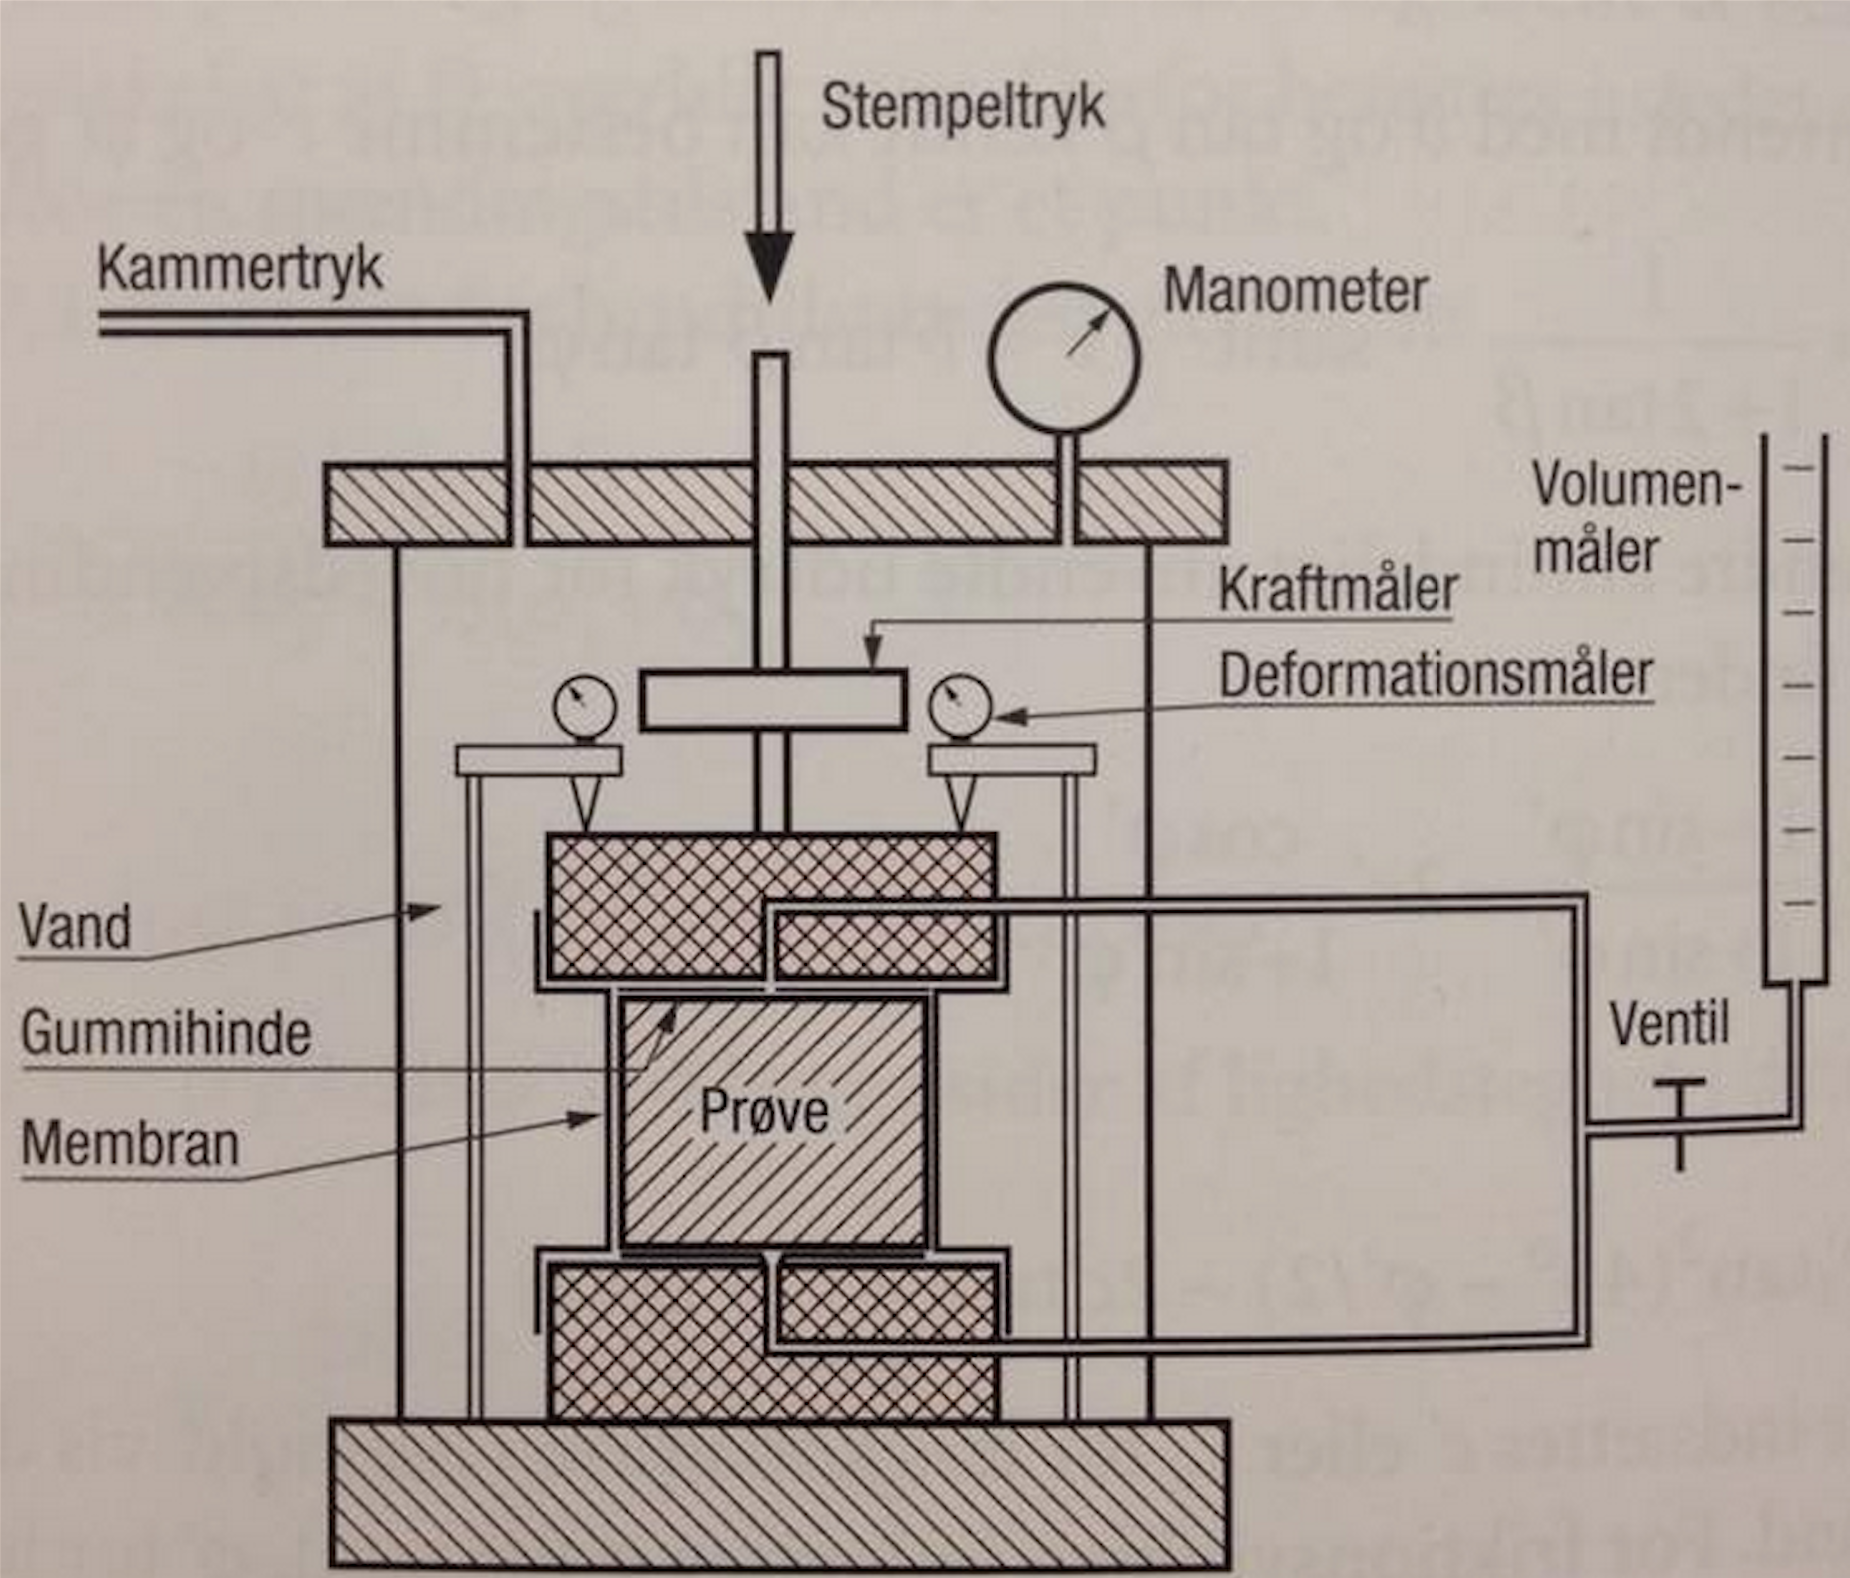
\includegraphics[width=0.6\textwidth]{billeder/forskud.png}
	\caption{triakselapparat \citep{geoteknik}}
	\label{fig:forskudningsspanding}
\end{figure}

\indent{     } 																																																																																																																																																																																						 Friktionsvinklen er et mål for jord styrke. Friktionsvinklen er vidt forskellige alt efter jordtype, hvilket er illustreret på Figur \ref{fig:friktionsvinkler}. Spændingernes størrelse har en betydning, da friktionsvinklen aftager med voksende spændinger. Der optræder også en kohæsion med disse spændinger, men dette er svært at regne i praksis, og derfor sættes \textit{c} (kohæsion) oftest lig nul ved eksempelvis sand. 

\begin{figure}[htbp]
	\centering
	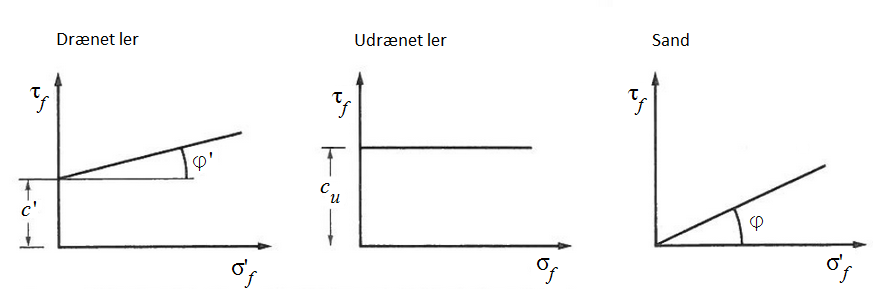
\includegraphics[width=1.0\textwidth]{billeder/friktionsvinkeller.png}
	\caption{Brudbetingelser for ler og sand \citep{geoteknik}}
	\label{fig:friktionsvinkler}
\end{figure}

\section{Aalborgs geologi}
Det danske landskab er overvejende formet under den sidste istid, Weichsel-istiden, der fandt sted for ca. 114.000-10.000 år siden. Under jordoverfladen findes bjergarter og aflejringer fra yngre tid end Weichsel-istiden. Det ældste i Danmarks dybder er grundfjeldet, bestående af granit og gnejs \citep{geopdf}, der anses for at ligge som en sokkel under Danmark og regnes for at være 1200-850 mio. år gammel. Over grundfjeldet findes aflejringer, der viser, hvordan klima, flora, fauna og jordskorpen har ændret sig de sidste ca. 500 mio. år samt hvordan hav og land skiftevis har haft indflydelse på området \citep{geolink}.
\newline
\newline
Kridttiden startede for 135 mio. år siden og sluttede igen for 65 mio. år siden. Kridttiden er opdelt i to perioder; Nedre- og Øvre Kridt, hvor Nedre Kridt strækker sig fra 135-100 mio. år siden, mens Øvre Kridt er fra 100-65 mio. år siden.  Øvre Kridt består hovedsageligt af skrivekridt \citep{geopdf}, som er en hvid bjergart, der let smitter af og indeholder store mængder kalk, ofte mellem 95 og 99,5\%. Kridtlagene er afsat på bunden af havet, som formodes at have haft en vanddybde på 100-250 m. Ved kridtlagets overflade findes såkaldte skorstene, der er skrå eller lodrette rør, ned gennem kridtlaget, fyldt med jord, som gør kridtlaget porøst \citep[ s. 15-16]{geobog}. Kridtlaget varierer i Danmark fra en tykkelse på 500 m til 2000 m.
\newline
\newline
Efter Kridttiden begyndte Tertiærtiden, der kan inddeles i flere underperioder, og som går fra år 65 mio. til 2,5 mio. før nu. Danien, også kaldet Nedre Paleocæn, dækker fra 65-62 mio. år før nu og minder om Øvre Kridt, da Danien også består af forskellige slags kalksten og flint. Der er dog den forskel, at Danien også indeholder forstenede dyr, hvilket Øvre Kridt ikke gør. Selve tykkelsen af Danien varierer fra 100 m til lidt over 200 m. Paleocæn dækker fra 62-55 mio. år siden. Dette lag indeholder meget ler, hvilket giver sedimenttypen mergel, når kalken eroderes. Øverst i Paleocæn befinder sig et lag af kalkfrit ler. Tykkelsen af Paleocæn for Danmark er vidt forskellig, men størst tykkelse findes på Midtsjælland, hvor der er 160 m. Mellem Nedre Paleocæn og Paleocæn findes et lag af bjergarten grønsandskalk, der er kalkrig, sand- og glauconitholdig.
\newline \indent{     }  Eocæn startede for 55 mio. år siden og sluttede 38 mio. før nu. Skellet fra Paleocæn og Eocæn består i et vulkanudbrud syd fra Norges sydkyst. Vulkanudbrudet afspejles i askelagene, som der findes 180 af, der tydeligt ses som mørke lag i det lyse moler, der består af ler og kiselskaller af encellede planter. Moleret er 50-60 m tyk for de vestlige egne af Limfjorden, mens den er 15 m tyk syd og sydøst for de vestlige egne af Limfjorden, og der er generelt meget tykke lag ler i det meste af Danmark \citep{geopdf}.
\newline
\newline
Kvartærtiden omfatter de sidste 2,5 mio. år tilbage og til nu og er kendetegnet ved store klimasvingninger mellem kolde og varme perioder. Weichselisen smeltede bort fra 22.000 år siden, hvilket markerede starten af den Senglaciale periode. Da den Senglaciale periode ophørte, var det meste af Danmarks nuværende landskab over havet. Undtaget var det nordligste af Jylland, hvor de smeltende gletcher skabte havstigning, som skyllede ind over området. Havet var et højarktisk ishav, som opstod da isen smeltede, og har fået navnet Yoldiahavet. I den sydlige og sydvestlige del af Vendsyssel blev Yoldiahavet afgrænset mod et aflejringsområde, der formodes at have været en stor smeltevandssø, hvori en skalfri leraflejring opstod. Denne leraflejring kaldes også for Aalborg ler og er en blød ler, der danner grundlag for Aalborg Midtbys geologi, som kun er let konsolideret af isen, hvorunder kridtlaget ligger. Først for ca. 13.000 år siden trak Yoldiahavet sig tilbage, efter at have lagt ind over Nordjylland i godt 2.000 år. Yoldiahavet blev trukket tilbage, da landskabet hævede sig, efter at have været tynget af isen, der nu var smeltet bort \citep{geopdf}.
\newline \indent{     }  Der er fundet frem til at Aalborg har et jordunderlag bestående af Aalborgler, som kun er blevet let konsolideret af istiden. Det risikerer derfor at  blive deformeret og derfor er det ikke et bæredygtigt jordunderlag. Dette betyder at der skal anvendes pælefundering ned til lag af jord, som er bæredygtigt. Dette tages der dog ikke højde for ,da der gerne vil arbejdes med direkte fundering i dette projekt, og vejleder har fundet boreprofiler fra Hals, som bliver beskrevet under. Dem laves der fundering ud fra. 


\section{Boreprofiler} 
I og med Aalborg har en undergrund primært bestående af Aalborgler, burde der anvendes pælefundering. Da der ønskes at arbejde med direkte fundering, tages der udgangspunkt i boreprofiler fra Hals, hvor undergrunden primært består af senglacialt sand, således det anvendte sand i forsøgene hænger sammen med de boreprofiler, som der ses på, da der ikke er sand i Aalborg Midtbys undergrund. Der ses på boring B17, som er vedlagt i Bilag F punkt 12.  
\newline \indent{     }  På boreprofil 17 ses, at grundvandsspejlet ligger omkring 0,8 m under overfladen. Der aflæses også, at undergrunden primært består af sand for boreprofilen. Via den stiplede linje aflæses vandindholdet i jordlaget. 
\newline \indent{     }  I boreprofil 16 i Bilag F punkt 11 findes et lag gytje mellem kote 2 og 3. Det ses, at vandindholdet i gytje er højere, samtidig med at modstanden i jordlaget ikke er højt. Når der funderes, skal der tages højde for denne svaghed i gytje, hvor der i nogle tilfælde vælges at grave laget væk, hvis gytjen ikke ligger for langt nede. Da den valgte boreprofil 17 ikke indeholder et lag af gytje, kan projektgruppen med fordel lave en direkte fundering.